\documentclass[12pt,english]{article}
\usepackage{mathptmx}

\usepackage{color}
\usepackage[dvipsnames]{xcolor}
\definecolor{darkblue}{RGB}{0.,0.,139.}

\usepackage[top=1in, bottom=1in, left=1in, right=1in]{geometry}
\usepackage{listings} 
\usepackage{amsmath}
\usepackage{amstext}
\usepackage{amssymb}
\usepackage{setspace}

\usepackage{graphicx}
\usepackage{float}

\usepackage[authoryear]{natbib}
\usepackage{url}
\usepackage{booktabs}
\usepackage[flushleft]{threeparttable}
\usepackage[english]{babel}
\usepackage{pdflscape}
\usepackage[unicode=true,pdfusetitle,
 bookmarks=true,bookmarksnumbered=false,bookmarksopen=false,
 breaklinks=true,pdfborder={0 0 0},backref=false,
 colorlinks,citecolor=black,filecolor=black,
 linkcolor=black,urlcolor=black]
 {hyperref}
\usepackage[all]{hypcap} % Links point to top of image, builds on hyperref
\usepackage{breakurl}    % Allows urls to wrap, including hyperref

\linespread{2}


% SETUP DOC ABOVE =============================================================
    \begin{document}
    
    \begin{singlespace}
    \title{Stock Portfolio Optimization and Automation Project}
    \end{singlespace}
    
    \author{Daniel Carpenter\thanks{University of Oklahoma.\
    E-mail~address:~\href{mailto:danielcarpenter@ou.edu}{danielcarpenter@ou.edu}}}

% \date{\today}
    \date{April 1, 2020}
    \maketitle
% ABSTRACT ====================================================================
    \begin{abstract}
    \begin{doublespace}
    	This paper will outline the methods and uses of a program that optimizes a stock portfolio. The portfolio consists of any stock that the user desires to include in the portfolio. The user can adjust the date range. If the tool is used for active portfolio management, the program suggests that the date range ends on the current date. The methods are based primarily on modern portfolio theory. This theory minimizes the risk of a portfolio, given the user’s desired return. The program uses a linear optimizer, which adjusts the weights of each stock to minimize the risk while setting the expected return to the user’s input. The program will output the stock weights, risk, and return characteristics, and some visualizations that aid the user in decision-making.
    
    \end{doublespace}
    \end{abstract}
    \vfill{}
    
    \pagebreak{}
    
%  START PAPER ================================================================
    \begin{doublespace}


    % INTRODUCTION ============================================================
    \section{Introduction}\label{sec:intro}\indent{}\indent{} % ---------------
    
       All individuals want to retire from their careers after some duration of time, but not all individuals can retire at the age that they desire. One may decide that their marginal propensity to consume satisfies their immediate needs and aspirations; however, focusing on delayed gratification will allow someone to foster realities like earlier retirement. As an individual who will soon enter the workplace, I know that I will also be eager to leave the workplace to enjoy the finer elements of my lifetime. While at The University of Oklahoma, my pursuit of a bachelor’s in business administration in Economics and Finance has motivated me to think critically about investing portions of my income. There are many forms of investments that someone may discover, but one of the more common are investments in the stock market. Many argue that the volatility of the stock market creates too much risk for individual investors, which their claims have validity within certain scopes (\citet{Zucker2020}). Corporate investors pay high premiums to minimize the time to trade on the stock market, which puts the individual investor at a disadvantage (\citet{Patter2020}). Although these circumstances hold, alternative investments may not be as liquid as stocks; if the investment is more liquid, such as a United States Treasury Bill, the “riskless” asset will not realize significant returns (\citet{Canady2020}). Note that the measurement of risk for stock analysis is the standard deviation of the historical unit, which the unit can range from stock prices, returns, or excess returns (\citet{Simon2008}). However, individual investors can minimize their risk when using certain financial methods. Within this paper, we will discuss how Modern Portfolio Theory allows an individual to minimize their risk of any portfolio, which can generate a return that satisfies the individual.  


    % LITERATURE REVIEW =======================================================
    \section{Literature Review}\label{sec:litreview}\indent{}\indent{} % ------
    
        Within this paper, combining the two concepts of Modern Portfolio Theory and the Capital Market Line underlines the financial principals that the program uses to optimize a stock portfolio. The reader may know the simple principle to “never put all your eggs into one basket;” Modern Portfolio Theory implements this idea using statistical methods and linear optimization to create a portfolio that maximizes utility and minimizes risk for an investor (\citet{Simon2008}). This method maximizes utility because it allows the investor to initially create their portfolio, given their preference in certain stocks (\citet{Simon2008}). Harry Markowitz announced this method is the 1950’s, who would receive a Nobel Prize in Economics in 1990 for the advancement of portfolio choice (\citet{Simon2008}). In addition to this idea, the Capital Market Line allows the user to allocate their optimal, or efficient, stock portfolio with “riskless” assets, such as the United States Treasury Bills (\citet{Simon2008}). The reader may find this discovery obvious, but the positive relationship between interest rate yields and the standard deviation of the yield commonly referred to as the risk of the asset, allows the Capital Allocation Line to easily reduce the risk, if the investor holds more weight in less risky assets (\citet{Simon2008}). 
        
        \indent{}\indent{} 
        Overall, these two ideas allowed investors to have more power over their portfolios; at the time of this discovery, individuals relied on their brokers to choose their stocks. This concept announced the allowance for “risk tolerance,” which the investor could best “fit their risk/reward profile” (\citet{Beatti2020}). However, these ideas are not commonly used by individual investors anymore; after extensive analysis, it is clear that “indexing,” which is a form of passive investing, outperforms “active” portfolio management (\citet{Malkie2017}). According to a study that the Wall Street Journal conducted, over 90 percent of actively managed portfolios underperform the S&P 500, which individuals can find indexes that combine the firms included in this value-weighted index fund (\citet{Malkie2017}). These index funds involve high-frequency trading tactics, which computer algorithms trade in fractions of a second; these machines are unbeatable by active portfolio managers, but individual investors may choose to index these funds to take part in the computerized gains (\citet{Patter2020}). Among these tactics, the introduction of artificial intelligence is at the forefront of portfolio management (\citet{Aenlle2018}). These implementations may allow for more powerful index funds, but full implementation of these ideas is not widely used yet (\citet{Aenlle2018}).
        
        \indent{}\indent{} 
        The user of this program must understand that actively managing a portfolio may not prove as successful as indexing, but it is important to understand that investors can establish preference that set their risk tolerance in the portfolio.


    % DATA ====================================================================
    \section{Data}\label{sec:data}\indent{}\indent{} % ------------------------
    
        \subsection{Using Yahoo Finance's API}
        The program uses one source of data, which houses stock-related information to the user. To allow for successful implementation of this program and continuous optimization of their stock portfolio, the use of the “BatchGetSymbols” package in R allows the user to have real-time data for any given stock. The package uses the API feature that Yahoo Finance allows to their constituents; Yahoo Finance’s allowance for API integration to their data provides seamless integration when applying the Modern Portfolio Theory. Not only can this package retrieve the most current data, but the user can also set the beginning period to their choice, which may prove valuable when wanting to consider only more recent periods. Within this program, the data includes month-end stock prices, which “BatchGetSymbols” will automatically calculate the monthly returns of the stock. See below graph for example of stock returns that the data automatically generates.
        
                \subsubsection{Figure 1: Example of Historical Returns using “BatchGetSymbols” package in R}
                    \begin{figure}[H]
                        \begin{center}
                            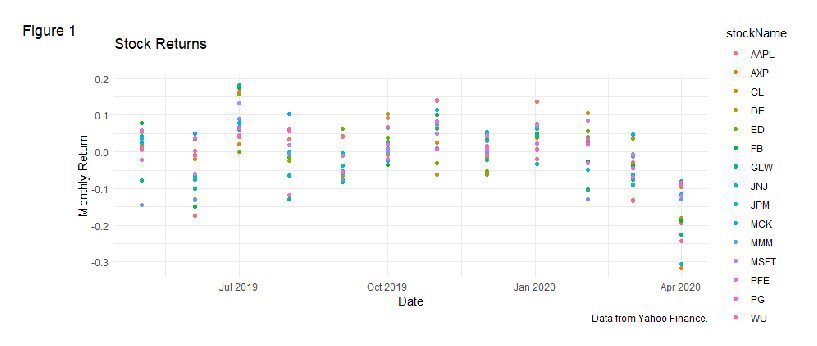
\includegraphics{FinalProject_Carpenter.eps}
                        \end{center}
                    \end{figure}
                
        Additionally, the user can select as many stocks as they would like to include in their portfolio. Conveniently, the package allows the operator to import the S&P 500, which is the optimization program’s default setting. This capability offers a vast span of the market, in which the optimization program can analyze and eliminate stocks that do not fit the user’s risk profile. An example of the data for stocks “JNJ,” “MSFT,” and “PG” from February through April 2020 can be seen below.
        
        \subsubsection{Table 1: Example of "BatchGetSymbols" API Export (Cleaned)}        
            \begin{center}
                % latex table generated in R 3.6.0 by xtable 1.8-4 package
                % Mon Apr 13 09:21:39 2020
                \begin{table}[H]
                \centering
                \begin{tabular}{rllrr}
                  \hline
                 & date & stockName & stockPrice & stockReturn \\ 
                  \hline
                1 & 2020-02-03 & JNJ & 149.22 & 0.03 \\ 
                  2 & 2020-03-02 & JNJ & 140.02 & -0.06 \\ 
                  3 & 2020-04-01 & JNJ & 128.81 & -0.08 \\ 
                  4 & 2020-02-03 & MSFT & 173.90 & 0.07 \\ 
                  5 & 2020-03-02 & MSFT & 172.79 & -0.01 \\ 
                  6 & 2020-04-01 & MSFT & 152.11 & -0.12 \\ 
                  7 & 2020-02-03 & PG & 125.11 & 0.01 \\ 
                  8 & 2020-03-02 & PG & 119.56 & -0.04 \\ 
                  9 & 2020-04-01 & PG & 109.33 & -0.09 \\ 
                   \hline
                \end{tabular}
                \end{table}
            \end{center}
        
        \subsection{Altering the Dataset}
        \indent{}\indent{}
        Once the optimization program successfully imports the dataset, it will manipulate the data to create the optimal format for the optimization portion of the program. The program will adjust aesthetic features, such as renaming the variables to a more familiar format. Additionally, the program will drop rows of the dataset that are null, which could be from the firm not having been publicly traded during the dates that the user selected, or it could be because of the dataset having null values in the stock return column. Further manipulation of the dataset occurs, which the “Empirical Methods” section covers in detail, due to the manipulation relying on statistical manipulation.


    % EMPIRICAL METHODS =======================================================
    \section{Empirical Methods}\label{sec:methods}\indent{}\indent{} % --------
    
        The optimization program uses financial and statistical methods to manipulate the dataset, which sets up the data for linear optimization. 
        
        % EXCESS RETURNS ------------------------------------------------------
        \subsection{Calculating Excess Returns}
        
    	    First, the program calculates excess returns for each stock.
                \begin{center}
                    \begin{equation} \label{Excess Returns}
                        Returns_{Excess} = Return_{Stock_{i}} - RiskFreeRate
                    \end{equation}
                \end{center}

            \indent{}\indent{}
            Calculating the excess return of a stock allows the user to understand what the stock returns beyond a riskless asset. The risk of an individual stock is measured by computing the standard deviation of the stock's excess returns. A common proxy for a “riskless” asset is the U.S. T-Bill, which is used in this analysis (\citet{Simon2008}). The use of this method is to understand the tradeoff between a riskless asset and another asset that bears greater risk. For example, if a stock returns less during a period on average than the U.S. T-Bill, which has little to no risk, then the investor should not take on more risk if there is no excess return. Remember that the relationship between risk and return is positive, in which the previous example would be negative (\citet{Simon2008}). Note that all calculations are per period, in which excess return should be denoted as the monthly-excess return within this analysis. 
        
        % VAR-COV-MATRIX ------------------------------------------------------
        \subsection{Calculating the Variance-Covariance Matrix}
        
            \indent{}\indent{}
        	The following method includes calculating the “Variance-Covariance Matrix,” which Benninga’s textbook, Financial Modelling, refers to as “central to all portfolio optimization” (\citet{Simon2008}). This matrix helps the program’s optimizer find the optimal weights that the investor should allocate to each stock. Broadly, this calculation discovers which stocks hold lower risk when implementing them into one portfolio (\citet{Simon2008}). 
            
            \indent{}\indent{}
        	The goal of this method is to understand how volatile an individual stock is, but it also will unveil increased risk of multiple stocks if they tend to “move” together (\citet{Simon2008}). Referring to the example of “putting your eggs into one basket,” this matrix shows which eggs to choose, which are coming from varying baskets. Continuing this example concerning the Variance-Covariance Matrix, if multiple baskets have a higher risk to be harmed at the same time as each other, then the Variance-Covariance Matrix will identify to the user which baskets should be removed. The calculation is as follows.
            
                \begin{center}
                    \begin{equation} \label{Variance-Covariance-Matrix}
                        Variance-Covariance-Matrix = 
                        \frac{X^{T}_{Excess Returns} \cdot X_{Excess Returns}}
                        {Number Of Stocks_{X_{Excess Returns}}} 
                    \end{equation}
               \end{center}
            
            \indent{}\indent{}
        	Using the stocks from Table 1 while increasing the date range to 10-years, the reader can view the Variance-Covariance Matrix for that portfolio below.
            
                
                \subsubsection{Table 2: Example of Variance-Covariance Matrix for Three-Stock Portfolio} 
                        % latex table generated in R 3.6.0 by xtable 1.8-4 package
                        % Mon Apr 13 10:00:10 2020
                        \begin{table}[H]
                        \centering
                        \begin{tabular}{rrrr}
                          \hline
                         & JNJ & MSFT & PG \\ 
                          \hline
                        JNJ & 0.04 & 0.03 & 0.02 \\ 
                          MSFT & 0.03 & 0.08 & 0.02 \\ 
                          PG & 0.02 & 0.02 & 0.04 \\ 
                           \hline
                        \end{tabular}
                        \end{table}
                    
                \indent{}
            	Within this matrix, the diagonal entries resemble the individual variances per stock; the off-diagonal entries show the covariance between two varying stocks (\citet{Simon2008}). If there is a higher covariance between certain stocks, then they have historically fluctuated in similar directions (\citet{Simon2008}). Notice that in this example, the diagonal entries are larger than the off-diagonal entries, which theoretically will always occur (\citet{Simon2008}). 

        % OPTIMIZE -------------------------------------------------------------
        \subsection{Optimizing the Weights of Each Stock in the Portfolio}
        
            \indent{}\indent{}
            After the program calculates the Variance-Covariance Matrix, the program will then use linear optimization techniques to minimize the risk of the portfolio, in which the equation is outlined in the following section, given the desired return an investor expects. Using the R package called “Rglpk,” the program will set the risk of the portfolio as its objective, in which it will minimize. The program will also set constraints on the optimization function, which will ensure that the combined weights of each stock add up to the portfolio’s 100 percent. For example, it is impossible to have 150 percent of our investment in some set of stocks; the allocation must not be greater than the investment. Another constraint is that the return must be greater than or equal to the user’s desired return. This assumption will allow for the package to minimize the risk of the portfolio, while still meeting a given return. Once the constraints have been satisfied, the package will give the program the optimal weights for each stock. Note that the user inputs the dollar amount of their investment, which in the case below is 10,000 dollars. See the following table for an example of the optimized output using an expanded set of stocks. Note that the sample has changed from the previous tables to simulate a more realistic version of the optimal portfolio.
            
            \subsubsection{Table 3: Optimized Portfolio Allocation}
                % latex table generated in R 3.6.0 by xtable 1.8-4 package
                % Wed Apr 29 12:49:40 2020
                \begin{table}[H]
                \centering
                \begin{tabular}{rlrr}
                  \hline
                 & Stock Name & Stock Weight & Dollar Investment \\ 
                  \hline
                1 & ADS & 0.47 & 4729.70 \\ 
                  2 & AMD & 0.53 & 5270.30 \\ 
                   \hline
                \end{tabular}
                \end{table}
                
            \indent{}
            Table 3 gives the optimal choice for a 6.00 percent expected return by allocating 4,729.70 dollars to ADS and 5,270.30 dollars to AMD.
                
        % RISK -----------------------------------------------------------------
        \subsection{Calculating the Risk of the Optimized Portfolio}
            
            \indent{}\indent{}
            Now that the program has optimized the weight of each stock in the portfolio, the program will calculate print the expected risk of the portfolio. It should be noted that the program has already calculated the risk so that it could minimize the equation; however, the program will validate the risk by printing the output to the user. If the portfolio included only a single stock, then the risk would simply be the standard deviation of the stock’s excess return. However, since a portfolio will typically include more than one stock, the program will use matrix algebra to compute this metric. Let the weights of each stock be a 1 x m vector, which includes the weight of each stock that the program optimized. The program multiplies this equation by the square root of 12, which provides the annualized risk for the portfolio. Given this vector and the Variance-Covariance Matrix, see the calculation of the risk below.
            
                \begin{center}
                    \begin{equation} \label{Portfolio Risk}
                        Risk_{Portfolio} = 
                        \sqrt{12} \cdot \sqrt{(StockWeights \cdot Variance-Covariance-Matrix) \cdot StockWeights^{T}}
                    \end{equation}
                \end{center}
        
        % RETURN ---------------------------------------------------------------
        \subsection{Calculating the Expected Return of the Optimized Portfolio} 

            \indent{}\indent{}
            To calculate the expected return of the portfolio, the program will use matrix multiplication to handle this problem. Calculating the return of the portfolio is a much simpler process than the risk of the portfolio. Conceptually, the program multiplies the stock weights by their respective expected returns, then adds these values to find the expected return of the portfolio. See the below equation for the expected return of a portfolio using matrix notation.
            	
                \begin{center}
                    \begin{equation} \label{Portfolio Return}
                        Return_{Portfolio} = 
                        12 \cdot StockWeights\cdot \overline{Return_{Stocks}}^{T}
                    \end{equation}
                \end{center}
        
        % SHARPE ---------------------------------------------------------------
        \subsection{Calculating the Sharpe Ratio of the Optimized Portfolio}

            \indent{}\indent{}
            The final calculation that the program performs is the Sharpe Ratio. The Sharpe Ratio is a measure of risk-adjusted returns. Explicitly, the measure gives the investor a value that shows the excess return per unit risk that they take by investing in this portfolio. The investor can compare Sharpe Ratio’s against another portfolio, which is a useful tactic when making investment decisions. The calculation of the Sharpe Ratio is below.
            	
                \begin{center}
                    \begin{equation} \label{Sharpe Ratio}
                        Sharpe_{Portfolio} = 
                        \frac{Return_{Portfolio} - RiskFreeRate}{Risk_{Portfolio}} 
                    \end{equation}
                \end{center}
                
            \indent{}
            Although investors commonly use the Sharpe Ratio, note that the main use is to compare this value to other portfolios that yield similar excess returns. For example, a portfolio that yields a very high yield and has relatively high risk may have a Sharpe Ratio that is higher than a portfolio with very low return and a small level of risk. Analysis of this method will vary between investors, based on their risk tolerance.
            
        \subsection{Summary Output of Risk, Return, and Sharpe Ratio}
            
            \indent{}\indent{}
            Below shows the final output of the risk, return, and Sharpe Ratio of the optimized portfolio, using the sample of stocks from Table 3. Note that the interpretation of risk is as follows. While setting the user's desired expected return to 6 percent, and given the historical excess returns for the portfolio's stocks, the expected variation in stock prices equals 5 percent. As mentioned, the portfolio expects a 6 percent return. Regarding the Sharpe Ratio, the portfolio takes on 0.81 units of risk per return, in excess of the risk free rate. All calculations are annualized.
            
            \subsubsection{Table 4: Summary Output of Risk, Return, and Sharpe Ratio of the Optimal Portfolio}
                % latex table generated in R 3.6.0 by xtable 1.8-4 package
                % Wed Apr 29 12:49:40 2020
                \begin{table}[H]
                \centering
                \begin{tabular}{rr}
                  \hline
                 & Value \\ 
                  \hline
                Risk & 0.05 \\ 
                  Expected Return & 0.06 \\ 
                  Sharpe Ratio & 0.81 \\ 
                   \hline
                \end{tabular}
                \end{table}
                
        \subsection{Summary Output of Upper and Lower Bounds of Portfolio Returns}
            
            \indent{}\indent{}
            Finally, the program will form a confidence interval around the expected portfolio returns, which will give the upper and lower bounds of the returns at a 95 percent confidence interval. For example, Table 5 shows the lower bound of returns equals 5.00 percent, while the upper bound totals 7.00 percent. Additionally, the program will tell the user the dollar amount that their investment will be given the lower and upper bounds.
    
            \subsubsection{Table 5: Summary of Upper and Lower Bounds of Portfolio Returns at 95 percent Confidence Level}
                % latex table generated in R 3.6.0 by xtable 1.8-4 package
                % Wed Apr 29 12:49:40 2020
                \begin{table}[H]
                \centering
                \begin{tabular}{rrr}
                  \hline
                 & Worst Case & Best Case \\ 
                  \hline
                Percent & 0.05 & 0.07 \\ 
                  Dollars & 10472.01 & 10727.99 \\ 
                   \hline
                \end{tabular}
                \end{table}

    % RESEARCH FINDINGS =======================================================
    \section{Research Findings}\label{sec:results}\indent{}\indent{} % --------
    
        Through the establishment of this tool, it is clear that passive index funds lead in superiority, compared to Modern Portfolio Theory. Although minimizing the risk of any portfolio does have validity in its fundamental nature, the competition of trading is fierce (\citet{Zucker2020}). Additionally, the active management of a portfolio may be costly in labor, which investment banks will charge minuscule rates on the return of a portfolio (\citet{Zucker2020}).
    
    % CONCLUSION ==============================================================
    \section{Conclusion}\label{sec:conclusion}\indent{}\indent{} % ------------
        The use of this program is to assist any investor in creating a stock portfolio and comparing these portfolios to other portfolios. As mentioned at the beginning of this paper, most individuals aspire to meet their retirement with plentiful amounts of wealth so that they may finish their lives with splendor and ease. Although indexing has crowded out Modern Portfolio Theory in many ways, this tool allows any investor to understand potential areas of investments, which require low levels of capital on the front end. Additionally, the high levels of liquidity that these assets offer give flexibility to the investor, which is a typical aspiration when pooling your funds into investments.
    
        \end{doublespace}
    
    % BIBLIOGRAPHY ============================================================
    
        \vfill
        \pagebreak{}
        \begin{spacing}{1.0}
        \bibliographystyle{jpe}
        \bibliography{FinalProject_Carpenter.bib}
        \addcontentsline{toc}{section}{References}
        \end{spacing}
        
        \vfill
        \pagebreak{}
        \clearpage
    
    % TABLES AND FIGURES =======================================================
    \newpage
    \section{Tables and Figures}
        \subsection{Figure 1: Example of Historical Returns using “BatchGetSymbols” package in R}
            \begin{figure}[H]
                \begin{center}
                    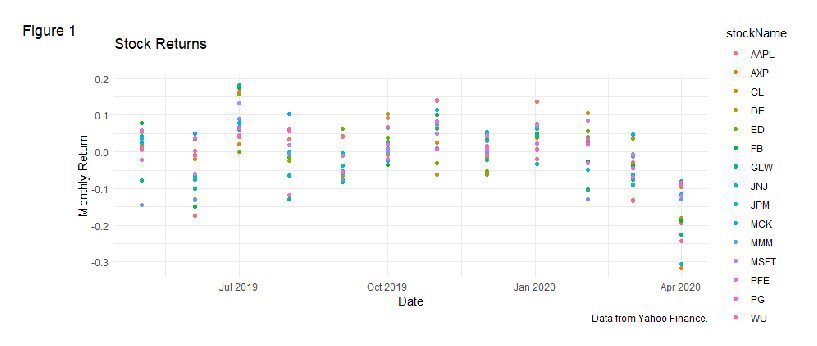
\includegraphics{FinalProject_Carpenter.eps}
                \end{center}
            \end{figure}
            
        \subsection{Table 1: Example of "BatchGetSymbols" API Export (Cleaned)}        
            \begin{center}
                % latex table generated in R 3.6.0 by xtable 1.8-4 package
                % Mon Apr 13 09:21:39 2020
                \begin{table}[H]
                \centering
                \begin{tabular}{rllrr}
                  \hline
                 & date & stockName & stockPrice & stockReturn \\ 
                  \hline
                1 & 2020-02-03 & JNJ & 149.22 & 0.03 \\ 
                  2 & 2020-03-02 & JNJ & 140.02 & -0.06 \\ 
                  3 & 2020-04-01 & JNJ & 128.81 & -0.08 \\ 
                  4 & 2020-02-03 & MSFT & 173.90 & 0.07 \\ 
                  5 & 2020-03-02 & MSFT & 172.79 & -0.01 \\ 
                  6 & 2020-04-01 & MSFT & 152.11 & -0.12 \\ 
                  7 & 2020-02-03 & PG & 125.11 & 0.01 \\ 
                  8 & 2020-03-02 & PG & 119.56 & -0.04 \\ 
                  9 & 2020-04-01 & PG & 109.33 & -0.09 \\ 
                   \hline
                \end{tabular}
                \end{table}
            \end{center}
        
        \subsection{Table 2: Example of Variance-Covariance Matrix for Three-Stock Portfolio} 
               % latex table generated in R 3.6.0 by xtable 1.8-4 package
               % Mon Apr 13 10:00:10 2020
                \begin{table}[H]
                \centering
                \begin{tabular}{rrrr}
                \hline
                 & JNJ & MSFT & PG \\ 
                \hline
                JNJ & 0.04 & 0.03 & 0.02 \\ 
                  MSFT & 0.03 & 0.08 & 0.02 \\ 
                  PG & 0.02 & 0.02 & 0.04 \\ 
                \hline
                \end{tabular}
                \end{table}
        
        \subsection{Table 3: Optimized Portfolio Allocation}
                % latex table generated in R 3.6.0 by xtable 1.8-4 package
                % Wed Apr 29 12:49:40 2020
                \begin{table}[H]
                \centering
                \begin{tabular}{rlrr}
                  \hline
                 & Stock Name & Stock Weight & Dollar Investment \\ 
                  \hline
                1 & ADS & 0.47 & 4729.70 \\ 
                  2 & AMD & 0.53 & 5270.30 \\ 
                   \hline
                \end{tabular}
                \end{table}
                
        \subsection{Table 4: Summary Output of Risk, Return, and Sharpe Ratio of the Optimal Portfolio}
                % latex table generated in R 3.6.0 by xtable 1.8-4 package
                % Wed Apr 29 12:49:40 2020
                \begin{table}[H]
                \centering
                \begin{tabular}{rr}
                  \hline
                 & Value \\ 
                  \hline
                Risk & 0.05 \\ 
                  Expected Return & 0.06 \\ 
                  Sharpe Ratio & 0.81 \\ 
                   \hline
                \end{tabular}
                \end{table}
                
        \subsection{Table 5: Summary of Upper and Lower Bounds of Portfolio Returns at 95 percent Confidence Level}
                % latex table generated in R 3.6.0 by xtable 1.8-4 package
                % Wed Apr 29 12:49:40 2020
                \begin{table}[H]
                \centering
                \begin{tabular}{rrr}
                  \hline
                 & Worst Case & Best Case \\ 
                  \hline
                Percent & 0.05 & 0.07 \\ 
                  Dollars & 10472.01 & 10727.99 \\ 
                   \hline
                \end{tabular}
                \end{table}
    
    % SOURCE CODE ==============================================================
    \newpage\section{Source Code}

    \lstset{basicstyle=\small,
            columns=fullflexible,
            frame=single,
            breaklines=true}

    \begin{singlespacing}    
        \lstinputlisting[language=R]{FinalProject_Carpenter.R}
    \end{singlespacing}
    
    \end{document}
